\ExamPart{Câu trắc nghiệm nhiều phương án lựa chọn}{3}{Mỗi câu hỏi thí sinh chỉ chọn một phương án.}

\NQuestion Cho hàm số $y=-x^2+4x+1$. Trục đối xứng của parabol là đường thẳng

\ChoicesOneLine{$x=2$.}{$x=-2$.}{$x=1$.}{$x=4$.}

\NQuestion Giá trị của $m$ để số $x=1$ là một nghiệm của phương trình $x^2+mx-2=0$ là

\ChoicesOneLine{$m=-1$.}{$m=1$.}{$m=2$.}{$m=-2$.}

\NQuestion Trong mặt phẳng tọa độ $Oxy$, phương trình đường thẳng đi qua điểm $A(1;2)$ và vuông góc với đường thẳng $d:2x-y+3=0$ là

\ChoicesTwoLines
{$x+2y-5=0$.}
{$2x-y=0$.}
{$x-2y+3=0$.}
{$2x+y-4=0$.}

\NQuestion Trong các điểm sau, điểm nào thuộc đường tròn $(C):(x-1)^2+(y+2)^2=9$?

\ChoicesTwoLines
{$M(4;-2)$.}
{$N(1;0)$.}
{$P(-1;-2)$.}
{$Q(2;0)$.}

\NQuestion Cho elip $(E):\dfrac{x^2}{64}+\dfrac{y^2}{9}=1$. Độ dài trục lớn của elip bằng

\ChoicesOneLine{$8$.}{$16$.}{$18$.}{$64$.}

\NQuestion Cho hàm số bậc hai $y=f\left(x\right)$ có đồ thị như hình dưới đây. Hàm số đồng biến trên khoảng nào?

\begin{center}
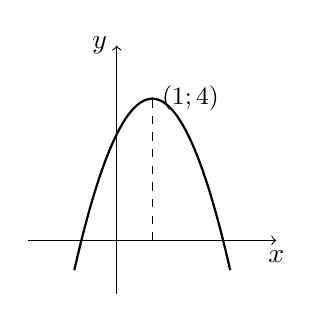
\begin{tikzpicture}[scale=0.45]
    \draw[->] (-2.5,0) -- (4.5,0) node[below] {$x$};
    \draw[->] (0,-1.5) -- (0,5.5) node[left] {$y$};

    \draw[dashed] (1,0) -- (1,4);
    \draw[thick, domain=-1.2:3.2, samples=200] plot (\x,{-((\x-1)^2)+4});

    \fill (1,4) circle (1.2pt);
    \node[right] at (1,4) {\small $(1;4)$};
\end{tikzpicture}

\end{center}

\ChoicesTwoLines
{$(-\infty;1)$.}
{$(1;+\infty)$.}
{$(-\infty;4)$.}
{$(4;+\infty)$.}

\NQuestion Cho đường tròn $(C):x^2+y^2-6x+4y+9=0$. Tọa độ tâm của đường tròn là

\ChoicesOneLine{$(3;-2)$.}{$(-3;2)$.}{$(3;2)$.}{$(-3;-2)$.}

\NQuestion Từ các chữ số $1,2,3,4,5$ có thể lập được bao nhiêu số tự nhiên lẻ gồm $3$ chữ số đôi một khác nhau?

\ChoicesOneLine{$24$.}{$36$.}{$48$.}{$60$.}

\NQuestion Trong mặt phẳng tọa độ $Oxy$, đường trung trực của đoạn thẳng $AB$ với $A(0;0)$, $B(4;2)$ có phương trình là

\ChoicesTwoLines
{$2x+y-5=0$.}
{$x-2y=0$.}
{$2x-y-5=0$.}
{$x+y-2=0$.}

\NQuestion Tập nghiệm của bất phương trình $(x-1)(x-4)\le 0$ là

\ChoicesTwoLines
{$[1;4]$.}
{$(-\infty;1]\cup[4;+\infty)$.}
{$(1;4)$.}
{$(-\infty;1)\cup(4;+\infty)$.}
